\section{Parking Lot Management System Architecture}

\begin{figure}[h!]
    \centering
    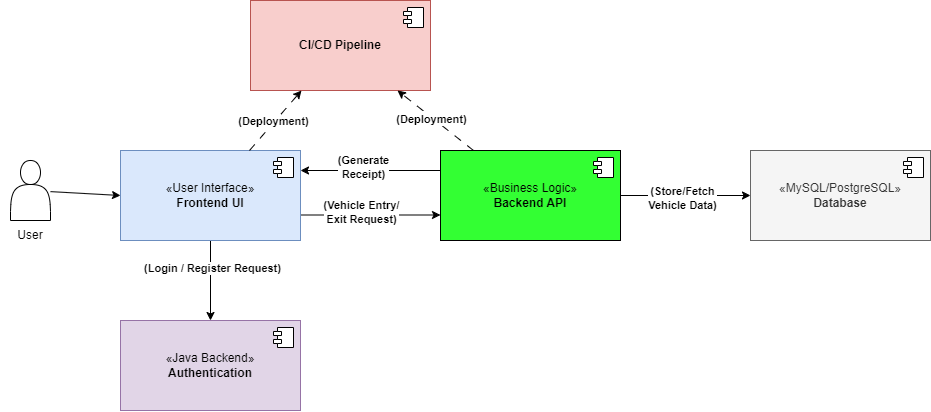
\includegraphics[width=1\textwidth]{Parking_Management_System_Architecture.png} % Ruta al archivo PDF con el diagrama
    \caption{UML Application Architecture Diagram for the Parking Management System}
    \label{fig:uml}
\end{figure}

The system consists of multiple components that work together to manage parking lot vehicle registration and receipt generation. Below is an explanation of the components and their roles in the system.

\begin{itemize}
    \item \textbf{User}: The Admin (such as a parking attendant) interacts with the system via the \textbf{Frontend UI} to log in and register vehicle entries and exits.
    \item \textbf{Frontend UI}: A user interface that enables the user to register vehicles entering and exiting the parking lot and generate receipts.
    \item \textbf{Business Logic (Backend API)}: This component handles all the logic related to vehicle entry/exit and receipt generation. It communicates with the database to store and fetch vehicle data.
    \item \textbf{Java Backend (Authentication)}: Manages user authentication (e.g., login and registration). It verifies user credentials with the database.
    \item \textbf{CI/CD Pipeline}: Automates the continuous integration and deployment process, ensuring that the system is always updated and tested before being deployed.
    \item \textbf{Database (MySQL/PostgreSQL)}: Stores data about vehicles, such as license plates, entry/exit times, and receipts.
\end{itemize}

\section*{Component Relationships}

The relationships between the components are as follows:

\begin{itemize}
    \item \textbf{User} $\to$ \textbf{Frontend UI}: The user interacts with the frontend for login and vehicle registration requests.
    \item \textbf{Frontend UI} $\to$ \textbf{Business Logic (Backend API)}: Sends vehicle registration and receipt generation requests to the backend.
    \item \textbf{Frontend UI} $\to$ \textbf{Java Backend (Authentication)}: Sends login requests to verify the user's credentials.
    \item \textbf{Business Logic (Backend API)} $\to$ \textbf{Database}: Stores and retrieves vehicle data (e.g., entry/exit times, receipt details).
    \item \textbf{CI/CD Pipeline} $\to$ \textbf{Frontend UI, Backend API}: Deploys updates automatically to the frontend and backend.
\end{itemize}
